\chapter{Алгоритам моделовања тема}

Сваким даном повећава се количина доступних дигиталних информација. Парадокс данашњег времена је да се упрокс великој количини података из различитих области све  теже долази до  података који су од интереса. Дакле, потребно је пронаћи алат којим би се велике количине података организовале а самим тим боље разумеле и лакше претреживале.

Тренутно, најпопуларнији начин претреге је према кључним речима. Кључне речи се предају неком систему за претрагу а као резултат добијамо скуп докумената који су повезани са њима. Иако овакав систем ради јако добро и са великом поузданошћу, постоје и другачији приступи % којима би се добили још бољи резултати. 

Најчешће питање које се поставља захтева одговр из неколико, ужих или ширих области. Међутим, кључне речи које се предају као критеријум претраге могу карактерисати и области које нису од интереса. На пример, Гугл претрга за кључне речи "ген, еволуција" ће у највећем броју случајема садржати веб странице посвећене биологији или сродним областима. Међутим, поменуте речи припадају и области рачунарства ( генетски алгоритми ) али ти резултати ће знатно слабије бити заступљени у односу на резултате везане за биологију. Тренутно се оваква врста проблема може решити додавањем још неке кључне речи која припада захтеваној области ( на пример за задате речи : алгоритам, кодирање, програм итд. ) међутим поствља се питање избора адекватних додатних речи, њихове заступљености у  захтеваној области као и релевантности у односу на друге кључне речи ( на примеру гугл претраге, често се дешава да механизам за претраживање испусти неку од речи и прикаже само резулатат за остатак упита )

Један од начина да се поменути проблем реши је и  претрага по тематици или теми докумената. Дакле, уместо претраге по кључним речима, најпре се пронађе област у  којој се врши претраживање а затим се  претражују докуменати који припадају тој области. На тај начин елиминишу се документи који би се у резултату појавили на основу предатих кључних речи али који нису повезани са  тематиком у којој се тражи одговор. 

На пример, нека је потребно пронаћи све чланке листа "Политика" у којима се говори о спортским успесима наше кошаркашке репрезантиције.Сви чланци овог листа могу се поделити у неколико категорија : политика, хроника, спорт, време итд. Пошто је од интереса категорија спорта, у обзир претраге долазе једино спортски чланци са тематиком  кошарке. На овај начин могуђе је пратити  како се мењао успех  кошаркашке репрезантиције са временом, колико се обаћала пажња на такве догађаје у ком временском периоду итд.

Описани вид претраге подразумевао би да се сваки лист "Политике" најпре прочита а затим  раздвоји по категоријама и "разуме" шта која категорија представља  како би се добили тражени подаци. Због велике количине података, овако нешто је немогуће урадити без помоћи рачунара. Алгоритми моделовања тема представљају први корак ка решавању оваквих и сродних проблема.

Циљ алгоритама за моделовање тема је "отривање" тема присутних у некој колекцији докумената. У суштини, алгоритми за моделовање су статистичке методе које на основу анализе свих речи у документу откривају које су то теме заступљене у том документу. За рад ове методе није потребно никакво претходно означавање докумената, теме докумената зависе једино од речи које се јављају у тексту. 

Моделовање тема омогућава организацију велике количине података на нивоу који је тешко дохватљив људским могућностима.

Надаље ће се паралелно употребљавати две еквивалентне ознаке - моделовање тема или ТМ ( скраћеница од енг. \textit{topic model})

\section{\textit{Latent Dirichlet allocation}}
 
\textit{Latent Dirichlet allocation}, надаље LDA, је најједноставнији приступ проблему моделовања тема \cite{blei1} а његова  примена била је и предмет овог рада.

Добро је познат роман Бранка Ћопића "Орлови рано лете". Уколико би неко ко није прочитао ови књигу желео да зна "о чему се ради" у њој, највероватније би добио одговор да је у питању књига која се бави доживљајима групе дечака на почетку Другог светског рата. Иако је то најшири оквир романа,у њему су присутне и теме о  љубави, дружењу, пријатељству, рату, пустоловинама итд.
Дакле, роман ,опште гледано, обухвата више тема, али се са неколико њих интензивно бави.

Уколико сада посматрамо овај рад као један пример документа, у њему се највише "говори" о моделовању тема и њиховој примени, али исто тако, само у мањој мери, и о  књижњвности ( пример књиге "Орлови рано лете " ).
Дакле, тешко је пронаћи било какав документ који се бави само једном темом. Чак се и у радовима који се баве неким уским научним областима, могу пронаћи делови који се могу сврстати и у неке друге научне области, било из исте, сродне или потпуно различите научне гране.

Основна претпоставка  LDA модела је управо да се сваки документ може сврстати у више области, тј. да се бави са неколико тема. 

Поставља се питање како то, да након читања неког документа, знамо да су у документу присутне различите теме и које су то теме. Уколико неки рад који се бави тематиком машинском учења прочита човек који се не бави рачунарством, највероватније је да би он као теме рада издвојио рачунарство и математику. Међутим, ако би исти рад прочитаоо неко ко се бави рачунарством, тада би он могао као потенцијалне теме да изведе једну или више области машинског учења, алгоритме, базе података, статистуку, теорију бројева итд. 
Дакле, издвојене теме зависе од "`знања"' онога ко чита рад. Уопштено, у оба случаја теме су издвојена на основу речи које се најчешчће срећу у областима које појединац познаје. Дакле, може се уопштити да тема представља \textbf{скуп карактеристичних речи.}. 

На следећој слици представљен је чланак "\textit{Seeking Life's Bare(Genetic) Necessities"} који "`говори о"' употреби анализе података за одређивање броја гена који организам треба да има да би преживео ( у еволутином смислу). Може се уочити да су три најзаступљеније области у овом тексту - анализа података, еволутивна биологија  и генетика. На њој су "ручно" означене неке речи које припдају овим областима. Речи које се могу сврстати у област \textit{анализе података} су означене плавом бојом, речи које припадају \textit{генетици} су означене жутом бојом док су речи које се односе на \textit{еволутивну биологију} означене розом бојом.
Уколико би се ова процедура применила на сваку реч текста, јасно би се уочило колико је која тема  заступљена у овом тексту. Математички, "\textit{присуство}" теме у тексту се означава односом  броја "обојених" речи у једну боју и укупног броја речи у тексту.

Наравно, постоје речи које се могу сврстати у више од једне теме. Такве речи ће бити обојене са две или више боја,али због прегледности слике, такви случајеви су изостављени.

\begin{figure}
    \centering
   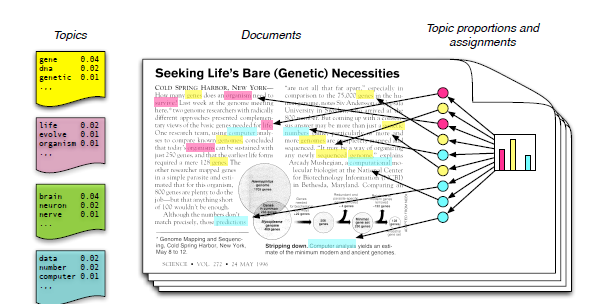
\includegraphics[scale=0.9]{./Slike/slika1.png} 
	\caption{Пример чланка, преузето са \cite{blei1}}
	\label{fig:slika1}
\end{figure}

На левој стани слике дате су неке теме ( енг. \textit{Topics}) које са одређеним вероватноћама садрже неке речи. На основу припадности речи темама, извршава се описани процес означавања ("бојења") речи да би се на крају добили удели тема у тексту ( десна страна слике, енг. \textit{Topics })
Важно је приметити да у тексту постоји доста речи које не одређују ни једну конкретну тему и које се са готово истим, малим вероватноћама могу сврстати у сваку од њих. Такве речи су нпр. везници, личне заменице ,прилошке одредбе итд. Оне се једним именом називају енг. \textit{stop words}. Како присуство таквих речи не утиче на тематику документа, то их при математичкој анализи текста треба занемарити.  



LDA је статистички модел који формално описује описани процес означавања речи. Да би се у потпуности разумело како LDA ради, потребно је упознати се са   \textit{генеративним процесом} -  процесом којим се креирају документи са становишта LDA-a.

\subsection{Генеративни процес}
Нека је дат неки скуп речи најчешће коришћених у научним областима математике, физике, хемије, музике, рачунарства и биологије. Нека је, даље, потребно креирати документ који има одређен број речи из датог скупа речи али тако да он највише "говори о"  математици и музици, али поред ових тема, у мањој мери, "говори о" физици и програмирању, док се остале теме занемарљиво мало помињу.
Како је дат фиксан скуп речи - речник (вокабулар ), могуће је свакој речи придружити \textit{вероватноћу} припадања свакој од тема. Тако ће на пример реч \textit{интеграл} имати велике вероватноће припадања темама математика и физика, мање вероватноће у темама хемија и рачунарство док ће се са јако малим вероватноћама јављати у осталим темама. Дакле, једна реч припада свакој од датих тема али са различитим вероватноћама. 

Генерисање траженог документа могуће је извести следећом процедуром :

\begin{enumerate}
 \item Одабрати расподелу тема у документу - прецизирати која тема се са којим уделом појављује у документу. У конкретном примеру, расподела би могла бити : математика 30\%, музика 30\%, физика 20\%,програмирање 15\%, биологија 2\% и хемија 3\%.
 \item Докле год није достигнут тражени број речи
 	\begin{enumerate}
	\item Изабрати тему из дистрибуције која је одабрана у 1.
	\item Изабрати реч из теме која је одабрана у 2.а). Како свака тема има речи које фаворизује ( веће вероватноће у односу на остале речи ), то ће се те речи највероватније одабрати у овом кораку.
	\end{enumerate}

 \end{enumerate}

Описана процедура може се графички илустровати претходном сликом (~\ref{fig:slika1}). Одабрана расподела тема у документу ( тачка 1 описане процедуре) предсављена је хистограмом на десној страни слике. Обојени кругови представљају одабир теме из документа ( корак 2.а) ) док речи повезане стралицама са њима представљају одабирану реч из те теме ( корак 2.б) ).\footnote{Расподела на основу које се одабирају пропорције тема у кораку 1, назива се Дирихлеова раподела, енг. Dirichlet distribution. На основу те одабране расподеле, врши се придруживање речи документима, енг. allocate } 

Формално, тема се дефинише као расподела речи над неким фиксним скупом речи - речником. Рецимо, тема биологија ће са већом вероватноћом садржати речи везане за ту област нпр. биљка, животиња, ћелија, ген итд. док ће тема везана за математику ове речи садржати са нижим вероватноћама у односу на речи нпр. број, разломак, променљива,коцка итд.


%PROVERI JOS JEDNOM DA LI MOZE TAKO DA SE KAZE

Дакле, основна карактеристика LDA-a је то што сви документи деле \textbf{исти скуп тема} али сваки документ те теме садржи у различитим односима. Овакаво посматрање докумената јако је природно и интуитивно.%{\color{red} Уколико би се могао формирати скуп свих речи које познаје нека особа, а затим тај скуп поделити по темама која та особа уме да разликује, механизам којим ће та особа препознати тематику докумената је у ствари начин на који LDA ради.} PROVERI!!!!

\subsection{Како се откривају теме - упрошћен пример }

Проликом генерисања поменутог документа, било је познато која тема садржи које речи као и у којим односима је заступљена свака тема у тексту. Циљ алгоритама за моделовање тема је да \textbf{аутоматски} "открије"  које су то теме присутне у неком документу и које речи припадају којој теми али \textbf{само} на основу речи које се јављају у документу, без било каквог додатног знања.
Сазнање о томе која тема се у којој мери налази у неком документу, није од превеликог практичног значаја. Међутим, уколико је на располагању огромна количина докумената ( нпр. дигитална база свих издаља листа "Политика" ), откривање сродних докумената, или докумената који се баве само одређеним темама може бити јако важно. Због тога ће се надаље говорити о скупу докумената над којим се извршава моделовање тема, уместо о једном документу. Притом, наравно, и даље важи претпоставка да сваки документ "говори о"   свим темама које се могу издвојити из свих докумената, само у различитим односима.

Према свему реченом, једино што је \textit{видљиво}, енг. \textbf{\textit{observed}} су документи, односно речи које се у документима јављају.  Тематска расподела по документима, као и расподела речи по темама су \textbf{\textit{скривене или невиљиве}}, енг.\textit{non observed,hidden} (Слика \ref{fig:slika2})

\begin{figure}[H]
    \centering
   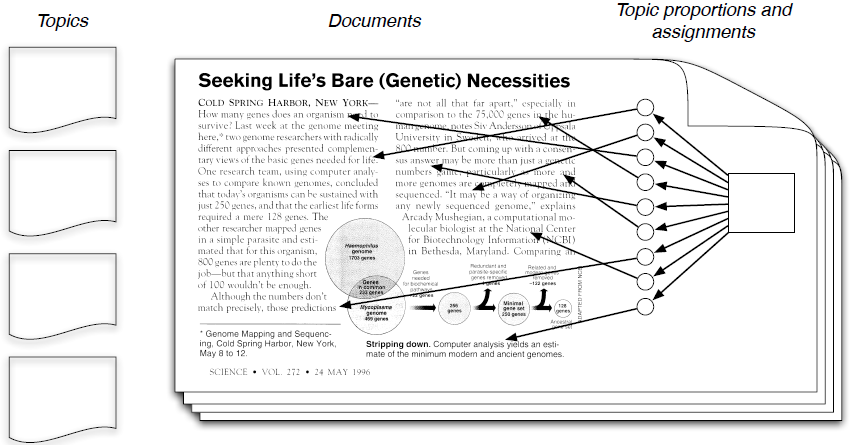
\includegraphics[scale=0.5]{./Slike/slika2.png} 
	\caption{Пример чланка, преузето са \cite{blei2}}
	\label{fig:slika2}
\end{figure}

Основни задатак алгоритма је окривање скривених структура на основу видљивих. У овом тренутку, моделовање тема можемо посматрати као \textbf{обрнути} генеративни процес. Дакле, циљ моделовања тема је откривање скривених структура из којих су \textbf{највероватније}, генеративним процесом, добијени видљиве структуре, тј. документи. Током рада, откривају се удели различитих тема по документима као и расподеле речи унутар тема.
Важно је напоменути да \textbf{именовање} тема не постоји у основној верзији алгоритма. Алгоритам групише речи у одређене целине - теме, а насловљавање тема се препушта стручњацима.




Нека је дат једноставан документ који, након склањања везника, личних заменица и осталих шумова (енг.\textit{stopwords}) садржи речи приказане у следећој табели.

\begin{figure}[H]
    \centering
   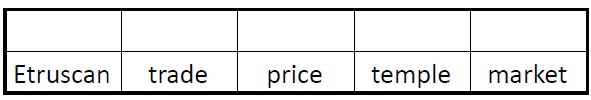
\includegraphics[scale=0.8]{./Slike/slika3.png} 
	\caption{Преузето са \cite{mimno1}}
	\label{fig:slika3}
\end{figure}

Процес моделовања тема започоње \textbf{случајним додељивањем} тема свакој од речи у документу. Дакле, пошто не постоји никакво знање о присуству тема у документима као ни о томе која реч припада којој теми, ову доделу је неопходно урадити на случајан начин. Интуитивно је јасно да се за тако нешто унапред мора одредити број тема који се захтева у задатом скупу докумената. Више о улазним параметрима алгоритма може се наћу у одељку 3 овог рада.
Пример једне случајне доделе дат је на следећој слици .
\begin{figure}[H]
    \centering
   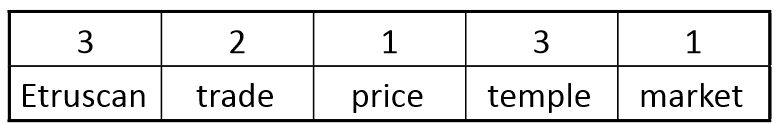
\includegraphics[scale=0.6]{./Slike/slika4.png} 
	\caption{Преузето са \cite{mimno1}}
	\label{fig:slika4}
\end{figure}

На овај начин је направљена иницијална \textbf{расподела} тема унутар посматраног документа - 40\% текста говори о теми 3, 40\% о теми 1, док 20\% говори о теми 2.

Уколико сада на сличан начин доделимо теме и осталим документима, полазни скуп докумената може се приказати следећом сликом.

\begin{figure}[H]
    \centering
   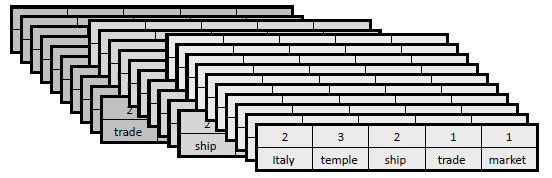
\includegraphics[scale=0.6]{./Slike/slika5.png} 
	\caption{Преузето са \cite{mimno1}}
	\label{fig:slika5}
\end{figure}

Пошто сваки документ има иницијалну, \textbf{случајну} расподелу тема, једноставно је груписати речи унутар тема и на тај начин направити иницијалну \textbf{случајну} расподелу речи по темама. Одређивање расподеле по темама, може се илустровати следећом сликом.


\begin{figure}[H]
    \centering
   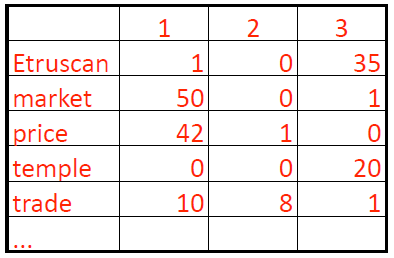
\includegraphics[scale=0.6]{./Slike/slika6.png} 
	\caption{Преузето са \cite{mimno1}}
	\label{fig:slika6}
\end{figure}
У првој колони табеле уписане су све речи из свих докумената (речник ) док је затим у свакој од наредних колона уписан одговарајући број који означава колико пута је дата реч додељена тој теми. Рецимо, бројеви 1 0 35 у другој врсти табеле означавају да је реч \textit{Etruscan} 35 пута била сврстана у тему број 3, једном је била додељена теми број 1 док се ниједним није нашла у теми број 2..
Дакле, почевши од друге колоне приказане табеле, табела по колонама, садржи  \textit{расподелу речи по темама}. Једноставним сортирањем колона, добијају се највероватније речи у свакој од тема.

У овом тренутку, расподеле које су добијене нису релевантне зато што у позадини стоји апсолутно случајно додељивање тема које није базирано на документима, тј. на јединим видљивим подацима.
Дакле, потребно је добијене резулатате \textit{прилагодити} тако да осликавају тематску структуру документа. Прилагођавање се одвија у одређеном, унапред познатом броју итерација. Генерално, што је већи број итерација, то су добијене расподеле релевантније, мада, како резултати показују, постоје и нека ограничења за ове вредности. Више о одређивању оптималног броја итерације може се наћи у одељцима 3 и 6 овог рада.

Унутар једне итерације, за сваки документ  за сваку реч унутар тог документа врши се провера колико је тренутно додељена тема адекватна, тј. да ли постоји боља тема којој би та реч могла бити додељена. На тај начин, из итерације у итерацију, расподеле све више и више осликавају структуру докумената.

Нека је почетна расподела по темама дата на претходним сликама (\ref{fig:slika5},\ref{fig:slika6}). Нека се провера подобности теме прво извршава за реч \textit{trade} првог документа. Ова реч је унутар првог документа додељена теми број 2, док је, гледано са становишта свих докумената који се посматтају, укупно 8 пута сврстана у ту тему. Потребно је испитати да ли тема број 2 највише одговара тој речи.
Претпоставимо да знамо теме за све остале речи, како из документа који се посматра, тако и за остале документе, и да је једино непозанто којој теми припада \textit{trade}  у посматраном документу.
Дакле, расподела тема у посматраном документу као и расподела речи по темама, сада изгледа као на следећој слици и потребно је доделити изабраној речи тему унутар посматраног документа.

\begin{figure}[H]
    \centering
   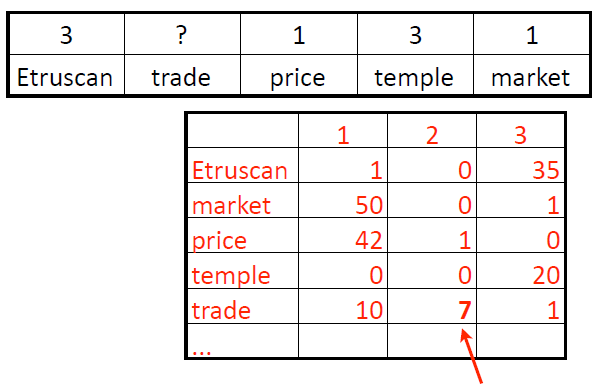
\includegraphics[scale=0.6]{./Slike/slika7.png} 
	\caption{Преузето са \cite{mimno1}}
	\label{fig:slika7}
\end{figure}

Уколико се посматра расподела тема у изабраном документу, приметиће се да документ највише "говори о"  темама 3 и 1 док о теми 2 не говори уопште. Према томе, удели тема 3 и 1 су значајни, док је удео теме 2 занемарљиво мали. Обзиром да је основна претпоставка овог модела да сви документи говоре о свим темама, не може се рећи да изабрани документ уопше "не говори" о теми 2. Начин на који ће се означити да је тема 2 јако слабо присутна у изабраном документу врши  се тако што се теми 2 додели јако мали удео. Обизиром да је у питању реч из документа који има неки одређену расподелиу тема, логично је очекивати да избор теме за ту реч зависи од тема тог документа.

Удели тема у изабраном документу могу се представити дужином линија, као што је приказано на следећој слици.


\begin{figure}[H]
    \centering
   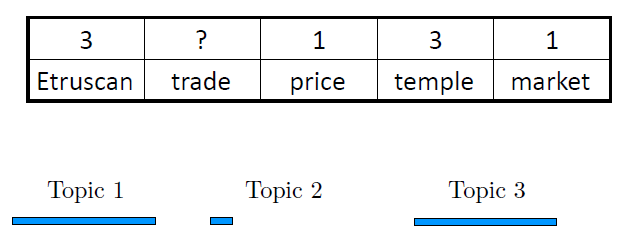
\includegraphics[scale=0.6]{./Slike/slika8.png} 
	\caption{Преузето са \cite{mimno1}}
	\label{fig:slika8}
\end{figure}

Међутим, како је речник ( скуп речи) заједнички за све документе, тема речи зависи и од глобалног присуства те речи у свим темама. И ова претпоставка је логична, јер, као што је на почетку наведено, свака реч припада свим темама, само са различитим вероватноћама. Глобално присуство изабране речи у свим темама приказано је на следећој слици :

\begin{figure}[H]
    \centering
   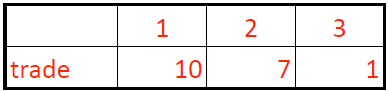
\includegraphics[scale=0.6]{./Slike/slika9.png} 
	\caption{Преузето са \cite{mimno1}}
	\label{fig:slika9}
\end{figure}


Дакле, избор теме за реч \textit{trade}  зависи од расподеле тема у посматраном документу као и од присуства те речи у свим темама. Ова зависност може се представити следећом сликом :

\begin{figure}[H]
    \centering
   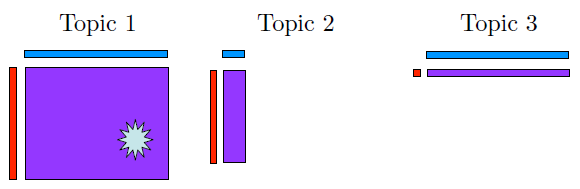
\includegraphics[scale=0.6]{./Slike/slika10.png} 
	\caption{Преузето са \cite{mimno1}}
	\label{fig:slika10}
\end{figure}

Вертикална, црвена линија представља присуство речи у одговарајучој теми ( формалније, вероватноћу са којом се та реч налази у изабраној теми ). Љубичаста "површина" представља подобност да одговарајућа тема буде додељена тој речи у изабраном документу. Како се слике јасно може уочити, "највећу"  површину формира тема 1 те је, према томе, речи  \textit{trade} додељује тема број 1 у овој итерацији. Након извршене измене, расподела тема у документу, као и расподела речи по темама, приказана је на следећој слици :



\begin{figure}[H]
    \centering
   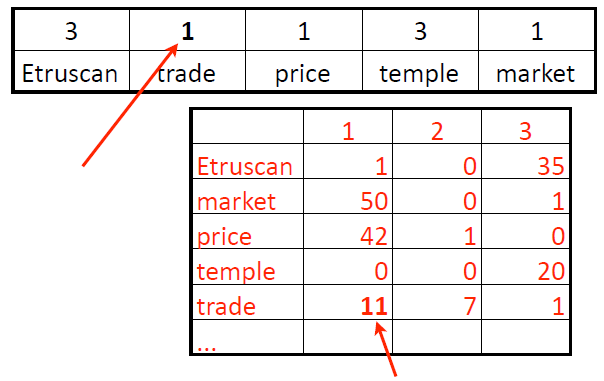
\includegraphics[scale=0.6]{./Slike/slika11.png} 
	\caption{Преузето са \cite{mimno1}}
	\label{fig:slika11}
\end{figure}


На овај начин, избараној речи додељена је најверпватнија тема а тематска слика документа "више личи" на реалну слику. 

Ако се описани процес примени на сваку реч сваког документа, расподеле ће из итерације у итерацију све више осликавати структуру полазних докумената. Обзиром да избор теме за сваку реч зависи од тренутно додљених расподела тема и речи, овим процесом се узимају у обзир видљиви подаци. Дакле, скривене структуре ( непознате расподеле) се генеришу на основу једино видљивих података - докумената и речи у њима.

Узевши све претходно у обзир, јасно је због чека не постоји именовање тема. Када се процес "генерисања"   заврши ( нпр. достигне  одређени број итерација ), сортирањем одговарајућих колона из табеле са слике \ref{fig:slika7}, добија се  расподела речи по темама. На основу експретског знања овим расподелама додељују се имена - нпр. тема 1 - математика, тема 2- економија итд.

%\subsection{Графички пример моделовања тема}
%
%Алгоритми за моделовање тема, поред текста, могу се применити и на друге облике података. Једна од могућих примена је и "`откривање тематике"' слика. Рецимо, помоћу ове групе алгоритама могуће је препознати "`сличне"' слике. Овај рад неће се бавити овом врстом примене, али се  ТМ алгоритама може јако добро илустровати једноставним графичким примером. Ради бољег разумевања шта ТМ уствари ради, биће описан један  пример примене ТМ над сликама.


%Нека је дат скуп једноставних слика, као што је приказано на 


























